% !TEX program = xelatex
\documentclass[a4paper,14pt,oneside,openany]{memoir}

%%% Задаем поля, отступы и межстрочный интервал %%%

\usepackage[left=30mm, right=15mm, top=20mm, bottom=20mm]{geometry}
\pagestyle{plain}
\parindent=1.25cm
\usepackage{indentfirst}

%%% Задаем языковые параметры и шрифт %%%

\usepackage[english,russian]{babel}
\babelfont[russian]{rm}{Times New Roman}
\babelfont[russian]{tt}{Courier New}

%%% Задаем стиль заголовков и подзаголовков в тексте %%%

\setsecnumdepth{subsection}
\renewcommand*{\chapterheadstart}{}
\renewcommand*{\printchaptername}{}
\renewcommand*{\chapnumfont}{\normalfont\bfseries}
\renewcommand*{\afterchapternum}{\hspace{1em}}
\renewcommand*{\printchaptertitle}[1]{\normalfont\bfseries\centering\MakeUppercase{#1}}
\setbeforesecskip{20pt}
\setaftersecskip{20pt}
\setsecheadstyle{\raggedright\normalfont\bfseries}
\setbeforesubsecskip{20pt}
\setaftersubsecskip{20pt}
\setsubsecheadstyle{\raggedright\normalfont\bfseries}

%%% Исправление нумерации секций %%%

\renewcommand{\thesection}{\arabic{section}}
\renewcommand{\thesubsection}{\arabic{subsection}}

%%% Сквозная нумерация рисунков и таблиц %%%

\counterwithout{figure}{chapter}
\counterwithout{table}{chapter}

%%% Выравнивание и переносы %%%

\tolerance 1414
\hbadness 1414
\emergencystretch 1.5em
\clubpenalty=10000
\widowpenalty=10000

%%% Задаем параметры оформления рисунков и таблиц %%%

\usepackage{graphicx}
\usepackage{caption}
\usepackage{subcaption}
\usepackage{float}
\graphicspath{{photo/}}
\captionsetup[figure]{font=small, width=\textwidth, name=Рисунок, justification=centering}
\captiondelim{ --- }
\usepackage[section]{placeins}

%%% Задаем параметры ссылок и гиперссылок %%% 

\usepackage{hyperref}
\hypersetup{
    colorlinks=true,
    linkcolor=red,
    citecolor=red
}

%%% Настраиваем отображение списков %%%

\usepackage{enumitem}
\renewcommand*{\labelitemi}{\normalfont{--}}
\setlist{noitemsep, leftmargin=*}

%%% Для verbatim %%%
\usepackage{verbatim}

\begin{document}

% Титульный лист (без номера страницы)
\thispagestyle{empty}

\begin{center}
    МИНИСТЕРСТВО ЦИФРОВОГО РАЗВИТИЯ, СВЯЗИ И МАССОВЫХ \\ КОММУНИКАЦИЙ \\ РОССИЙСКОЙ ФЕДЕРАЦИИ

    \vspace{20pt}

    Федеральное государственное бюджетное образовательное учреждение \\ высшего образования \\
    "Сибирский государственный университет телекоммуникаций и \\ информатики"

    \vspace{20pt}

    Кафедра телекоммуникационных систем и вычислительных средств \\ (ТС и ВС)
\end{center}

\vfill

\begin{center}
    Практическая работа №6 \\
    по дисциплине \\
    \textit{"Web-технологии"}

    \vspace{20pt}

    по теме: \\
    \uppercase{Облачное файловое хранилище Seafile}
\end{center}

\vfill

\noindent Студент: \\
\textit{Группа ИКС-532 \hfill Шиф Д.А.}

\vspace{20pt}

\noindent Преподаватель: \\
\textit{старший преподаватель \hfill А.В. Андреев}

\vfill

\begin{center}
    Новосибирск 2026 г.
\end{center}

\newpage
\setcounter{page}{2}
\OnehalfSpacing*

\subsection*{Цель работы}

\begin{itemize}
    \item Развернуть облачное файловое хранилище Seafile на отдельной виртуальной машине
    \item Настроить статический IP-адрес и DNS-запись для сервера Seafile
    \item Настроить веб-сервер Nginx в качестве Reverse Proxy
\end{itemize}

\section{Введение}

В данной практической работе настраивается облачное файловое хранилище Seafile на отдельной виртуальной машине. Seafile позволяет организовать синхронизацию файлов между клиентами локальной сети, предоставляя доступ через веб-интерфейс и клиентские приложения.

Параметры варианта:
\begin{itemize}
    \item Номер варианта: 20
    \item Подсеть: 192.168.20.0/24
    \item Домен: SHIF.20.internal
    \item IP-адрес сервера Seafile: 192.168.20.4
    \item IP-адрес шлюза: 192.168.20.1
\end{itemize}

\section{Ход работы}

\subsection{Создание и настройка виртуальной машины Seafile}

Была создана виртуальная машина с именем seafile в Oracle VirtualBox. Параметры ВМ:
\begin{itemize}
    \item Операционная система: Ubuntu 22.04.5 LTS
    \item Оперативная память: 2048 МБ
    \item Жесткий диск: 25 ГБ (динамический VDI)
    \item Сетевой адаптер: Внутренняя сеть (intnet)
\end{itemize}

Настройка статического IP-адреса выполнена в файле \texttt{/etc/netplan/00-installer-config.yaml}:

\begin{verbatim}
network:
  version: 2
  renderer: networkd
  ethernets:
    enp0s3:
      dhcp4: no
      addresses:
        - 192.168.20.4/24
      routes:
        - to: default
          via: 192.168.20.1
      nameservers:
        addresses: [192.168.20.1, 8.8.8.8]
        search: [SHIF.20.internal]
\end{verbatim}

\begin{figure}[H]
    \centering
    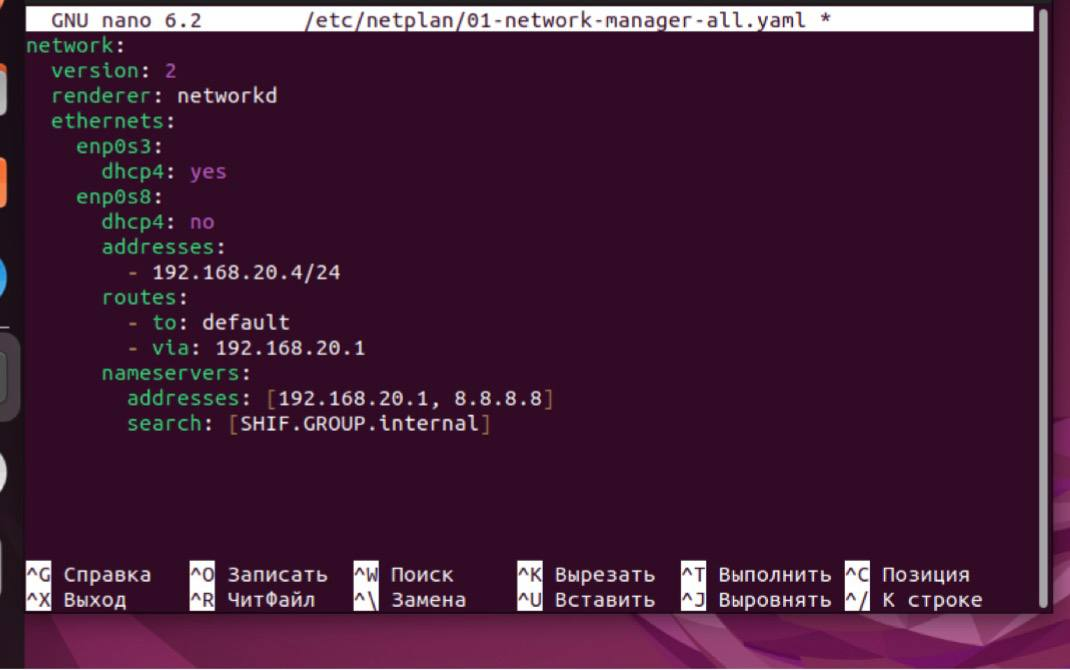
\includegraphics[width=0.7\textwidth]{111.jpg}
    \caption{Настройка сетевого интерфейса ВМ seafile}
\end{figure}

\subsection{Добавление DNS-записи на шлюзе}

На сервере gateway (192.168.20.1) в файл прямой зоны добавлена A-запись:

\begin{verbatim}
seafile IN A 192.168.20.4
\end{verbatim}

\begin{figure}[H]
    \centering
    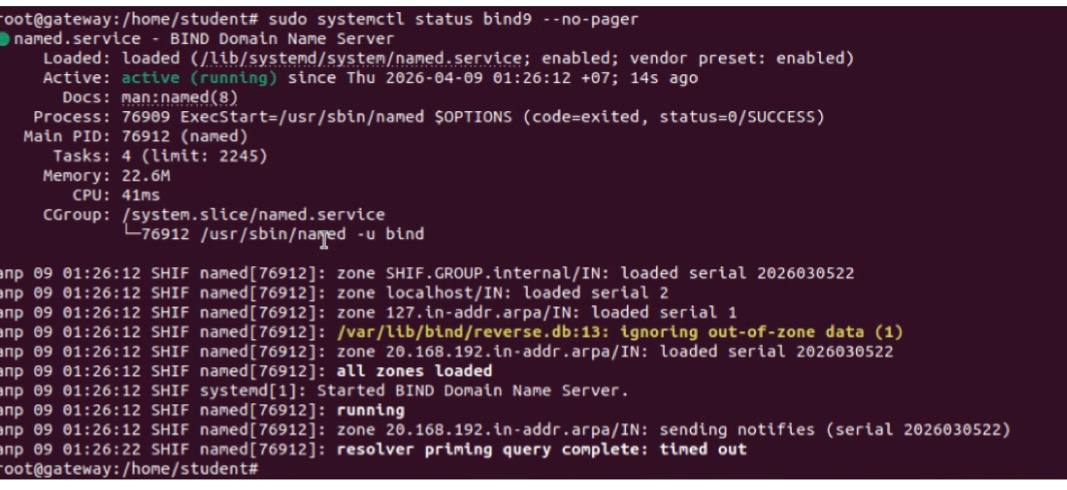
\includegraphics[width=0.7\textwidth]{222.jpg}
    \caption{Добавление DNS-записи в файл forward.db}
\end{figure}

\subsection{Установка Seafile и настройка Nginx}

После установки Seafile был настроен веб-сервер Nginx для проксирования запросов на порт 8000. Конфигурационный файл \texttt{/etc/nginx/sites-available/seafile.conf}:

\begin{verbatim}
server {
    listen 80;
    server_name seafile.SHIF.20.internal;
    
    location / {
        proxy_pass http://127.0.0.1:8000;
        proxy_set_header Host $host;
        proxy_set_header X-Real-IP $remote_addr;
        proxy_set_header X-Forwarded-For $proxy_add_x_forwarded_for;
        proxy_buffering off;
    }
}
\end{verbatim}

\section{Результат работы}

Сервер успешно запущен и доступен по адресу \texttt{http://seafile.SHIF.20.internal}. Веб-интерфейс Seafile работает корректно.

\section*{Заключение}
\addcontentsline{toc}{section}{Заключение}

В ходе работы было развернуто облачное хранилище Seafile, настроен статический IP, DNS-запись и Reverse Proxy через Nginx. Задачи выполнены в полном объеме.

\end{document}